\documentclass[12pt]{beamer}
\usetheme{Madrid}

\usepackage{amsmath, amsfonts}
\usepackage{hyperref}
\usepackage[super,comma,numbers]{natbib}
\renewcommand{\bibnumfmt}[1]{[#1]}
\bibliographystyle{apsrev4-1}

\title{Semi-permeable membranes as domain walls}
\author[A. Brown]{Aiyan B.}
\date{December 23, 2025}

\newcommand{\abs}[1]{\left| #1 \right|} % | |
\newcommand{\avg}[1]{\left\langle #1 \right\rangle} % < >

\begin{document}

\maketitle

\begin{frame}{Semi-permeable membranes as domain walls}
    \begin{itemize}
        \item Consider a 1d lattice of spacing $a > 0$.
        The lattice is separated by placing a semi-permeable membrane between sites $M$ and $M+1$~\cite{Das_2023},
        which can be crossed with probability $\lambda < 1/2$
        \item On the left of the membrane consists of a media with temporal step size $\tau_l$ and on the right a media with step size $\tau_r$ 
        -- eventually amounting to varying diffusivities
    \end{itemize}
    \begin{figure}
        \centering
        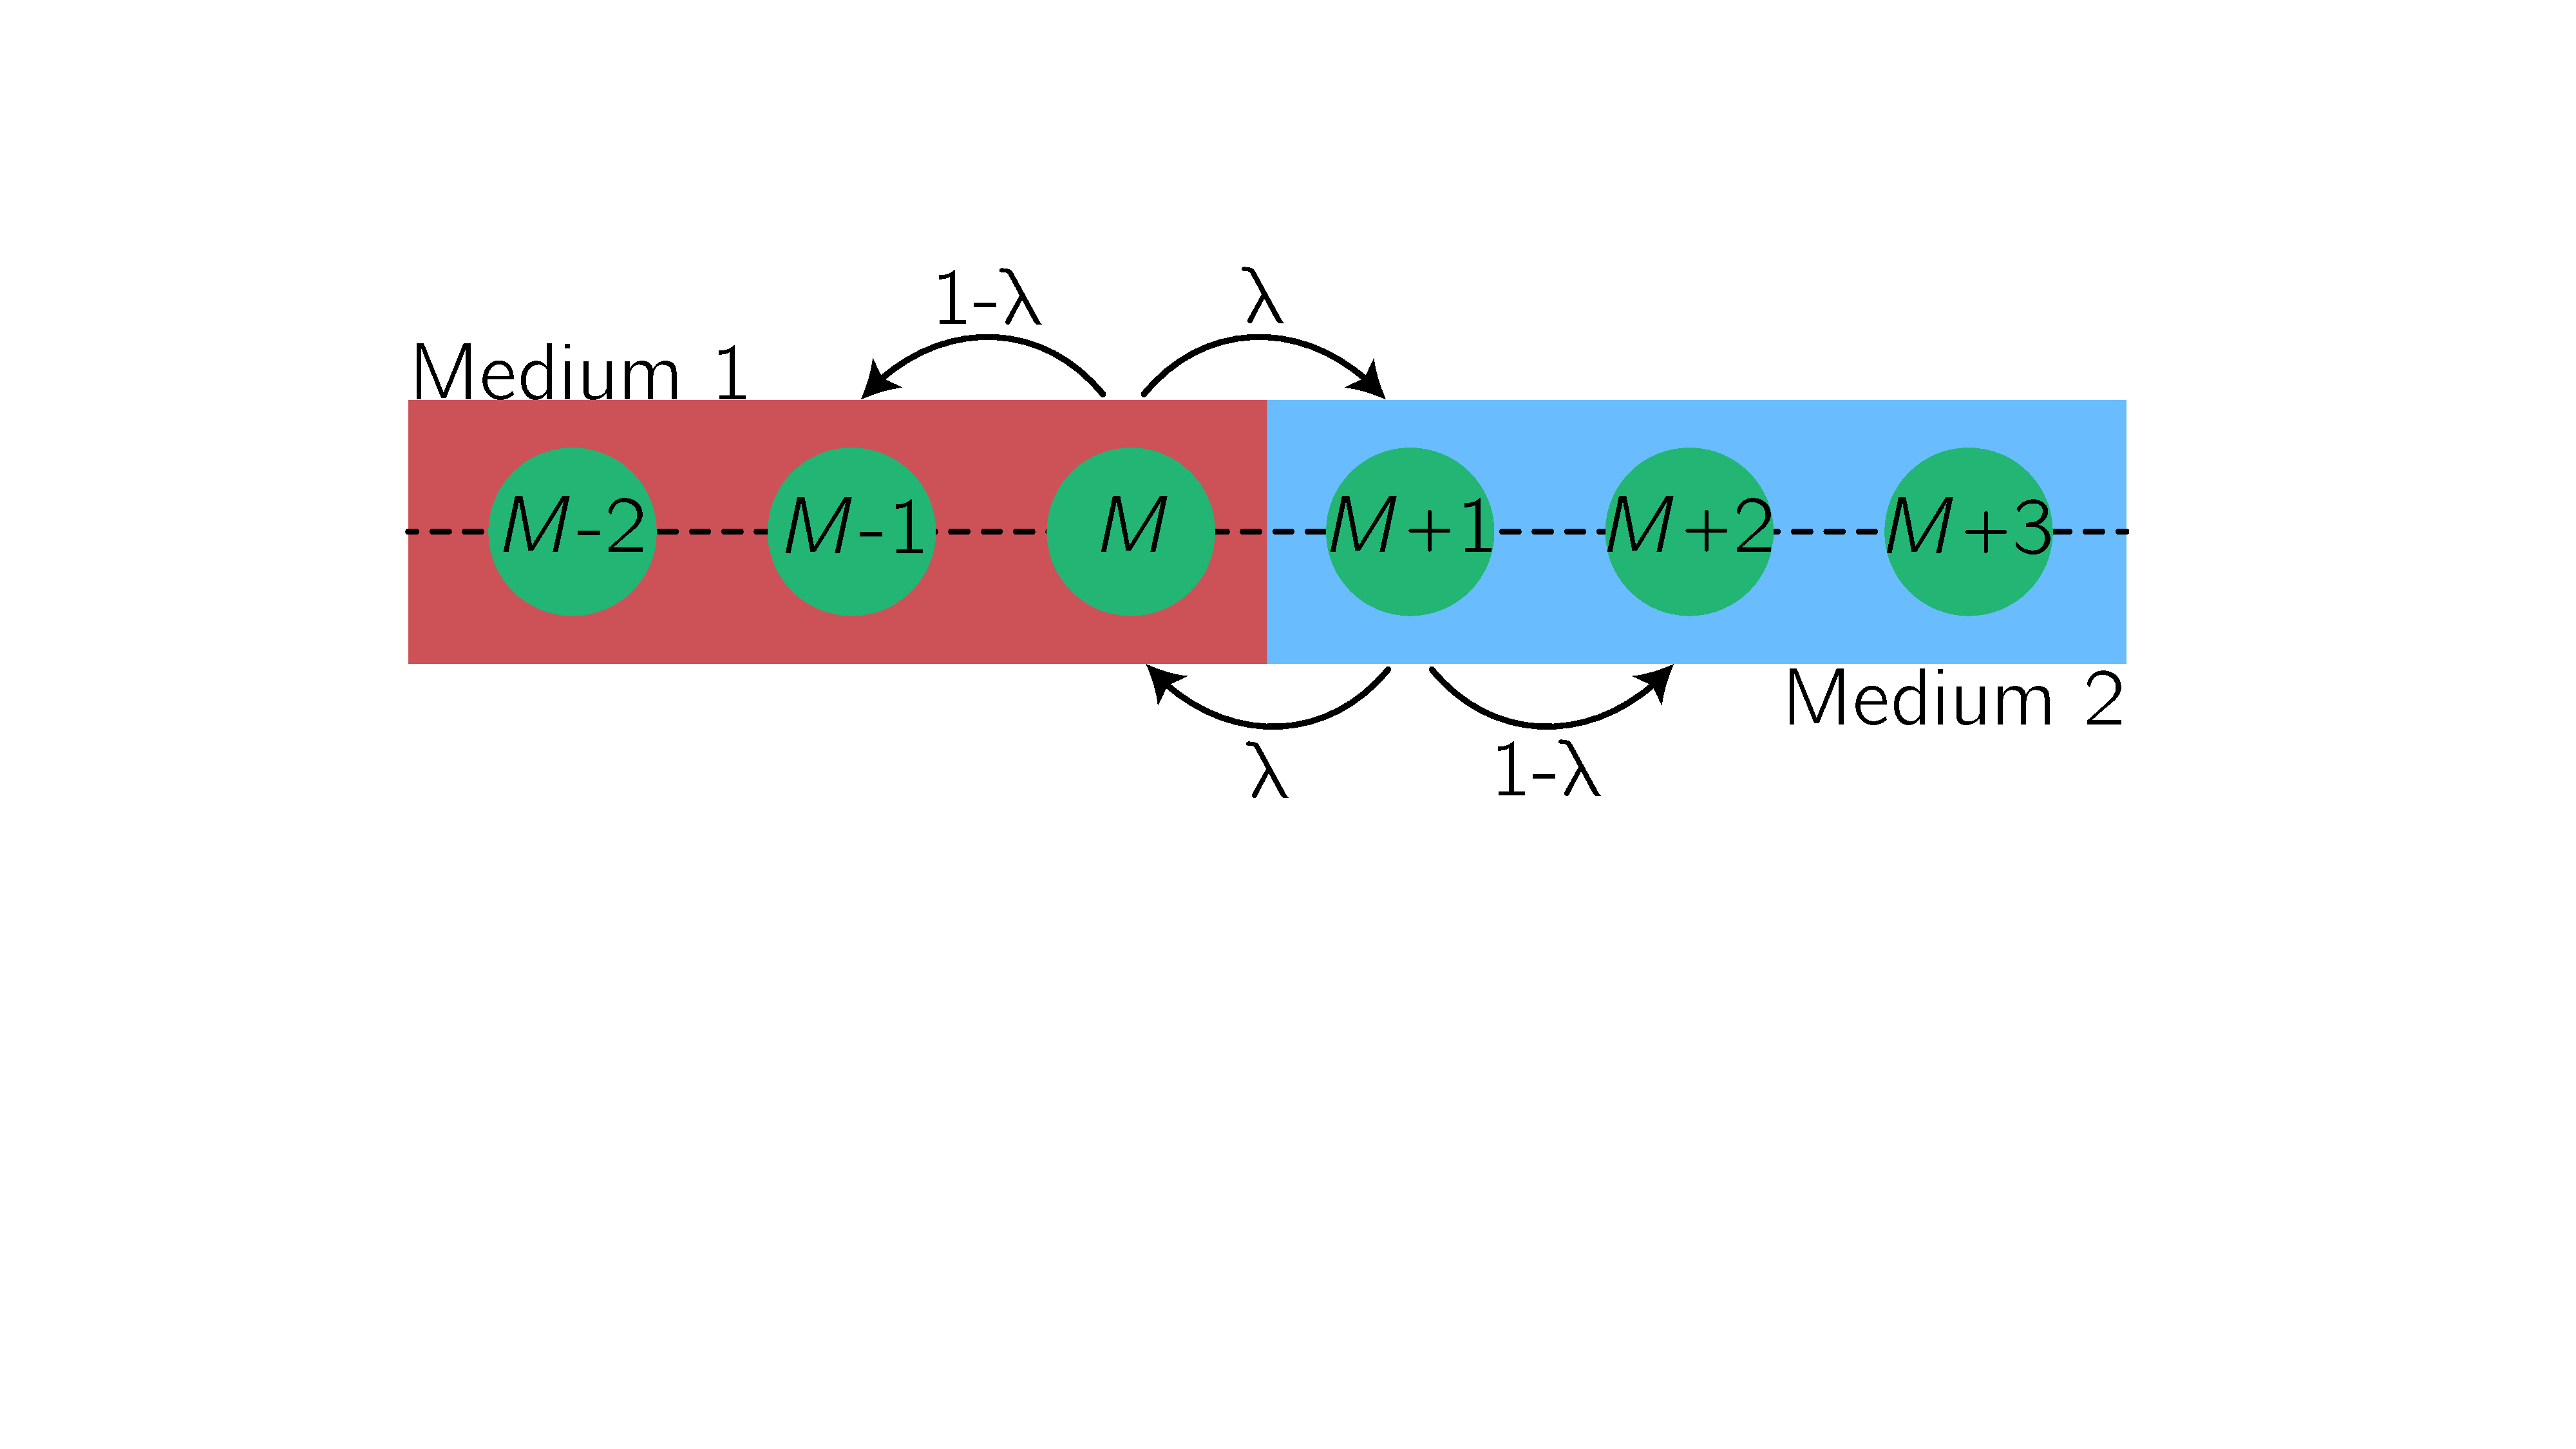
\includegraphics[width=0.9\textwidth]{figures/model.pdf}
    \end{figure}
\end{frame}

\begin{frame}{The master equation}
    \begin{itemize}
        \item Let $p_j (t)$ denote the probability of being at site $j$ at time $t$ and $\Delta = \frac{1}{2} - \lambda$.
        The (global) master equation for the system reads
    \end{itemize}
    \begin{multline} \label{eq:1}
        \frac{\partial p_j (t)}{\partial t} 
        = \left[ \frac{1}{2} p_{j + 1} + \frac{1}{2} p_{j - 1} - p_j  \right] 
        \left( \frac{1}{\tau_l} \sum_{k = - \infty}^M \delta_{j, k} + \frac{1}{\tau_r} \sum_{k = M+1}^\infty \delta_{j, k} \right) \\
        + \frac{\Delta}{\tau_l} p_M (t) \delta_{j, M-1} 
        + \frac{\Delta}{\tau_r} p_{M+1} (t) \delta_{j, M + 2} \\
        + \left( \frac{\lambda}{\tau_r} - \frac{1}{2 \tau_l} \right) p_{M+1} (t) \delta_{j,M}
        + \left( \frac{\lambda}{\tau_l} - \frac{1}{2 \tau_r} \right) p_M (t) \delta_{j,M+1}
    \end{multline}
\end{frame}

\begin{frame}{The continuum limit}
    \begin{itemize}
        \item Consider the discrete-to-continuum mapping, 
        $p_j (t) \to p (x,t)$, $M \to x_b$, $D_i = a^2 / 2 \tau_i$ and $\delta_{j,k} \to a \delta (x - y)$
        \pause
        \item Keep terms to $\mathcal{O} (a^4)$ and let the \textbf{reluctivity} of the media, 
        $\nu_i = \frac{4 (2 \lambda - 1) \tau_i}{a}$, remain finite
        in the limit $a \to 0$,
    \end{itemize}
    \begin{multline} \label{eq:2}
        \frac{\partial p}{\partial t} 
        = \frac{\partial}{\partial x} \left[ D(x) \frac{\partial p}{\partial x} \right]
        + \left( 4 \lambda - 1 \right) \left( D_r - D_l \right) p (x_b, t) \delta' (x - x_b) \\ 
        - D_r^2 \nu_r \frac{\partial p (x_b, t)}{\partial x} \delta' (x - x_b),
    \end{multline}
    where $D(x) = D_l \Theta(x_b-x) + D_r \Theta (x-x_b)$ is the state-dependent diffusivity
    \pause
    \begin{itemize}
        \item When $D_r = D_l$, diffusion becomes homogeneous across membrane 
        and we recover Kay \& Giuggioli (2022)~\cite{Kay2022}
        \item When $\lambda = 1/2$, $\nu_r \to 0$ and the third term on RHS vanishes
    \end{itemize}
\end{frame}

\begin{frame}{Replacing deltas with BCs}
    \begin{itemize}
        \item We can write the right-hand side of Eq.~\eqref{eq:2} in terms of a generalized probability flux,
        \begin{equation} \label{eq:3}
            J (x,t) = 
            - D (x) \partial_x p(x,t) 
            - \chi (t) \delta (x - x_b),
        \end{equation}
        which satisfies the continuity equation $\partial_t p + \partial_x J = 0$
        \pause
        \item Can then use the piecewise continuity of $p$ to show that we can equivalently 
        write Eq.~\eqref{eq:2} $\partial_t p = \partial_x \left( D(x) \partial_x p \right)$ with the boundary conditions
        (i) $J$ is everywhere continuous and (ii) obeys the self-consistency condition
        \begin{equation} \label{eq:4}
            D (x_b) [p (x_b,t)]
            = (4 \lambda - 1) (D_r - D_l) p (x_b, t) 
            - D_r^2 \nu_r \frac{\partial p (x_b, t)}{\partial x},
        \end{equation}
        where $[p(x_b, t)] := p_r (x_b^+, t) - p_l (x_b^-, t)$
    \end{itemize}
\end{frame}

\begin{frame}{A FPE interpretation}
    \begin{itemize}
        \item The Dirac delta is the distribution satisfying $\langle \delta_a, \varphi \rangle = \varphi (a)$ for a test function $\varphi$
        \pause
        \item Differential operator acts on distributions as 
        $\langle \delta_a', \varphi \rangle = - \langle \delta_a, \varphi' \rangle = - \varphi' (a)$ so
        $\delta'(x - a) f(a) = \delta (x - a) \partial_x f (x) + \delta'(x-a) f (x)$ leading to
    \end{itemize}
    \begin{equation}
        \frac{\partial p}{\partial t} = - \frac{\partial}{\partial x} \left[ \mu(x, t) p (x,t) \right]
        + \frac{\partial^2}{\partial x^2} \left[ \sigma (x, t) p (x,t) \right]
    \end{equation}
    for drift
    \begin{equation*}
        \mu (x,t) = 
        \frac{\partial D}{\partial x} 
        + (4 \lambda - 1) (D_r - D_l) \delta (x - x_b) 
        - D_r^2 \nu_r \delta'(x - x_b)
    \end{equation*}
    and effective diffusivity 
    \begin{equation*}
        \sigma (x,t) = D(x) - D_r^2 \nu_r \delta (x - x_b)
    \end{equation*}
\end{frame}

\begin{frame}{The case of many domains}
    \begin{itemize}
        \item Membranes are specified by 3-tuples $\{ (x_i, \lambda_i, D_i) \}$, for $x_{i+1} > x_i$,
        containing their position, probability of crossing, and diffusivity in the domain between $x_{i-1}$ and $x_i$, respectively
        -- satisfying $x_0 = - \infty$, $x_{\max{i}} = + \infty$ and $\lambda_{\max{i}} = 0$:
    \end{itemize}
    \begin{multline*}
        \frac{\partial p (x, t)}{\partial t} 
        = \frac{\partial}{\partial x} \left[ 
            \sum_i D_i \left[ \Theta (x-x_{i-1}) - \Theta (x-x_i) \right] 
            \frac{\partial p (x,t)}{\partial x} 
        \right] \\
        + \sum_i \left[ 
            \left( 4 \lambda_i - 1 \right) \left( D_{i+1} - D_i \right) p (x_i, t)
            - D_{i+1}^2 \nu_{i+1} \frac{\partial p (x_b, t)}{\partial x}
        \right] \delta' (x - x_i),
    \end{multline*}
    \vspace{-10pt}
    \pause
    \begin{figure}
        \centering
        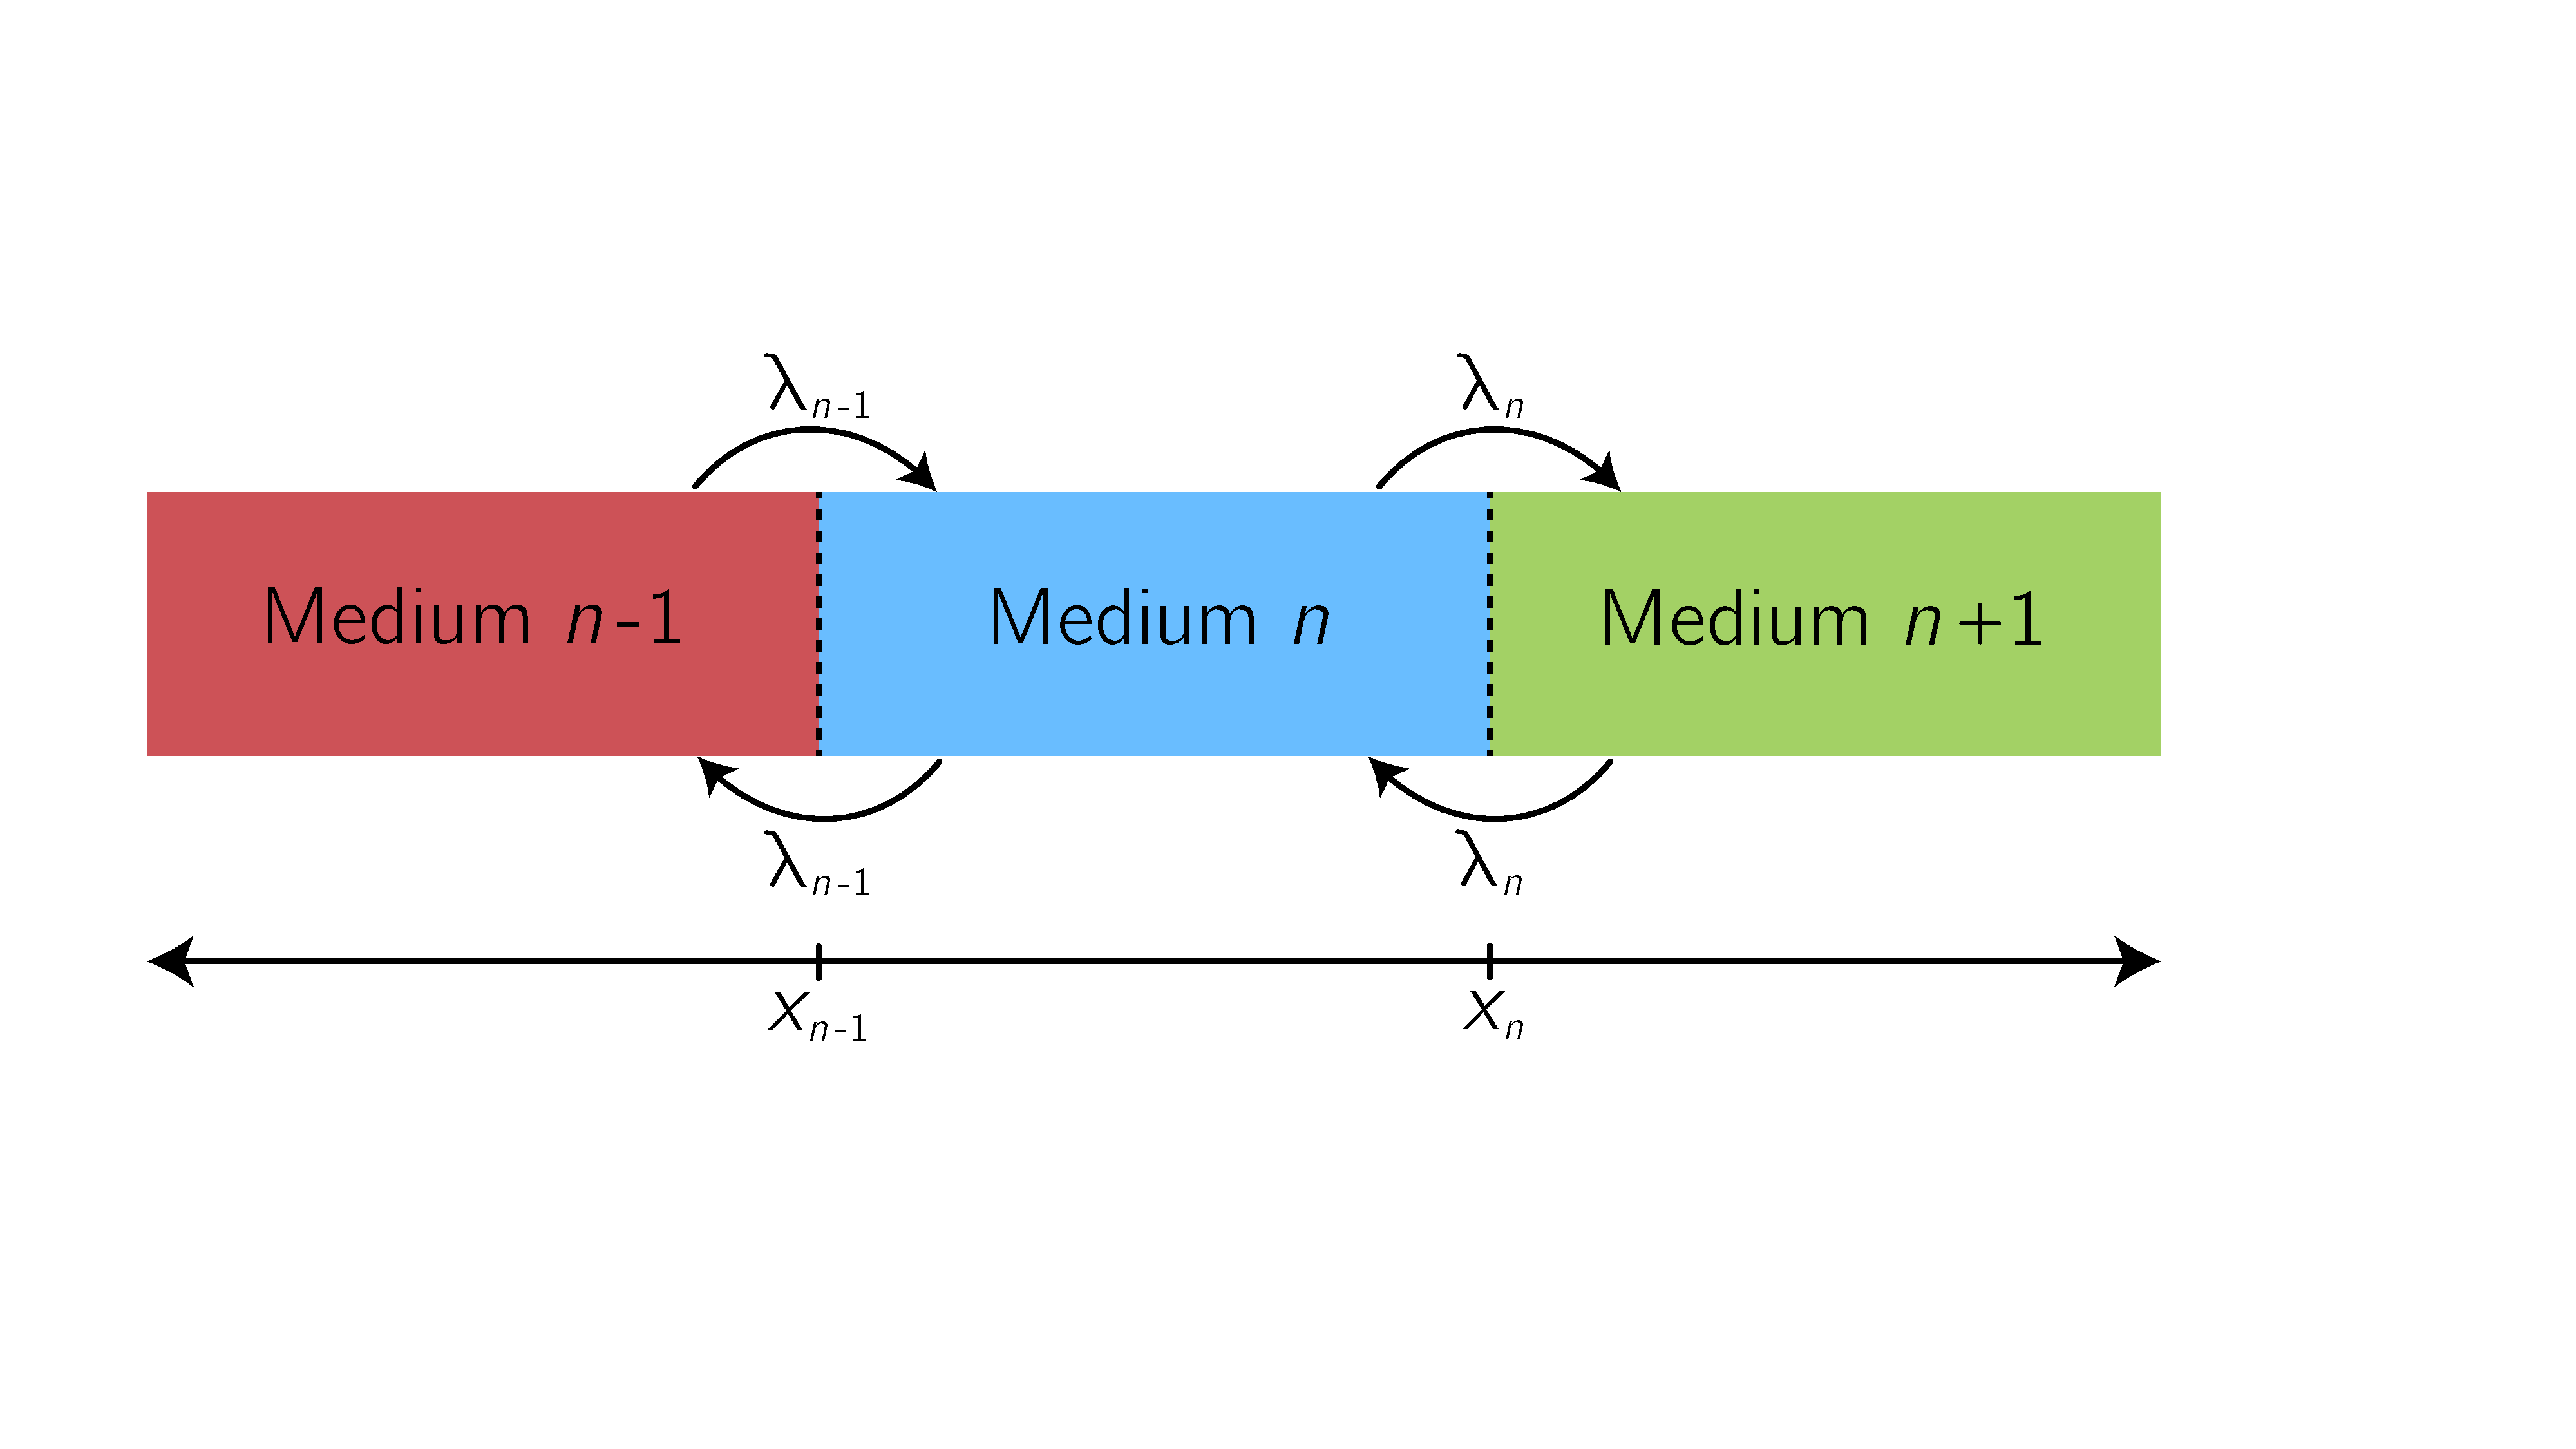
\includegraphics[width=0.7\textwidth]{figures/many-model.pdf}
    \end{figure}
\end{frame}

\begin{frame}{Some natural questions}
    \begin{enumerate}
        \item What is the first passage time within a given domain?
        \pause
        \item What is the MSD for this model, given some statistical behaviour for $\{ (x_i, \lambda_i, D_i) \}$?
        \pause
        \begin{enumerate}
            \item What are the minimum conditions for anomalous diffusion?
            \item What are the minimum conditions process ergodicity?
        \end{enumerate}
        \pause
        \item What is the long-time, effective diffusivity $K_\alpha$, $\avg{x^2 (t)} = 2 K_\alpha t^\alpha$?
        Are there distinct behaviours depending on values of $\nu_i$?
        \pause
        \item How many times, on average, does a particle cross a membrane at time $t$?
        \item How much time is spent ``at'' the membrane?
    \end{enumerate}
\end{frame}

\begin{frame}{A probabilistic approach}
    \begin{itemize}
        \item Choose to constrain each of the parameters probabilistically~\cite{PhysRevLett.112.150603}
        \pause
        \begin{enumerate}
            \item Consider the membrane reluctivity $\nu$ 
            for a given domain as the ``fundamental'' scaling. 
            We impose a lower limit $\Lambda > 0$ to ensure generically non-trivial behaviour and suppose that the
            probability density of the reluctivity scales as 
            $p_\nu (\nu) \sim \abs{\nu - \Lambda}^{- \alpha}$ for $\alpha > 0$ and $\nu \sim \Lambda$
            \pause
            \item Given the reluctivity $\nu$ in a domain, 
            diffusivity and domain size, $r_i = x_i - x_{i-1}$, 
            are (conditionally) independent and PDFs depend on reluctivity as 
            $p (\cdot \mid \nu) = f (\nu / \Lambda)$ for some function $f$
        \end{enumerate}
        \item The joint PDF can be written as 
        \begin{equation*}
            p (\nu, r, D) = p_\nu (\nu) p_D (D \mid \nu) p_\nu (D \mid \nu)
        \end{equation*}
        \pause
        \item If $x(t)$ has (i) uncorrelated increments and (ii) $\avg{x^2 (t)} \sim t^\beta$,
        then the process has non-stationary increments and shows weak ergodicity breaking~\cite{PhysRevLett.112.150603}
    \end{itemize}
\end{frame}

\begin{frame}{References}
    \bibliography{references}
\end{frame}

\begin{frame}{The continuum limit I}
    \begin{multline}
        \frac{\partial p (x, t)}{\partial t} 
        = \left[ D_l \Theta(x_b-x) + D_r \Theta (x-x_b) \right] \frac{\partial^2 p (x,t)}{\partial x^2} \\
        + a \frac{\Delta}{\tau_l} p (x_b, t) \delta (x - (x_b - a))
        + a \frac{\Delta}{\tau_r} p (x_b + a, t) \delta (x - (x_b + 2 a)) \\
        + a \left( \frac{\lambda}{\tau_r} - \frac{1}{2 \tau_l} \right) p (x_b + a, t) \delta (x - x_b) \\
        + a \left( \frac{\lambda}{\tau_l} - \frac{1}{2 \tau_r} \right) p (x_b, t) \delta (x - (x_b + a))
    \end{multline}
\end{frame}

\begin{frame}{The continuum limit II}
    \begin{multline}
        \frac{\partial p (x, t)}{\partial t} 
        = \left[ D_l \Theta(x_b-x) + D_r \Theta (x-x_b) \right] \frac{\partial^2 p (x,t)}{\partial x^2} \\
        + a^2 \left( 2 \lambda - \frac{1}{2} \right) p (x_b, t) \delta' (x - x_b) \left( \frac{1}{\tau_r} - \frac{1}{\tau_l} \right) \\
        + \frac{a^2}{2} \left( \frac{1}{\tau_r} - \frac{1}{\tau_l} \right) \frac{\partial p (x_b, t)}{\partial x} \delta (x - x_b) \\
        + \frac{a^3}{4} \left( \frac{1}{\tau_r} - \frac{1}{\tau_l} \right) \left[ \frac{\partial p (x_b, t)}{\partial x} \delta (x - x_b) - p (x_b, t) \delta '' (x - x_b) \right] \\
        - \frac{a^3}{\tau_r} \left( 2 \lambda - 1 \right) \frac{\partial p (x_b, t)}{\partial x} \delta' (x - x_b) + \mathcal{O} (a^4)
    \end{multline}
    \begin{itemize}
        \item The fourth term vanishes as $\tau \sim a^2$ and there is no additional coupling
    \end{itemize}
\end{frame}

\begin{frame}{On the unphysicality of the reluctivity}
    In defining a non-trivial membrane, we take
    \begin{equation*}
        \nu = \lim_{\tau, a \to 0} \frac{4 \tau (2 \lambda - 1)}{a} 
        = \lim_{a \to 0} \frac{2 a}{D} (2 \lambda - 1)
    \end{equation*}
    to remain finite, positive and non-zero unless $\lambda = 1/2$.
    If we constrain $\lambda \in [0,1]$, this is clearly impossible, necessitating that we let
    \begin{equation*}
        \lambda (a) = \frac{1}{2} + \frac{c}{a},
    \end{equation*}
    where $c$ is defined such that the limit is $\nu$.
    As the lattice spacing becomes vanishingly small, 
    the necessity of the divergence of $\lambda$ arises from the unphysical nature of the membrane:  
    it only influences an infinitesimal volume, which can only have a
    finite effect if the local flow is infinite.
\end{frame}

\begin{frame}{Moments}
    \begin{itemize}
        \item The mean moments of the distribution can be found by integrating with respect to $p(x,t)$.
        Using Eq.~\eqref{eq:2}, can determine the rate of change of these moments as 
        \begin{equation}
            \frac{d \avg{x^n (t)}}{dt} = \int_{- \infty}^\infty x^n \frac{\partial p (x,t)}{\partial t} \, dx
        \end{equation}
        \item To first and second order, with $\varsigma = D_r - D_l$,
        \begin{subequations}
            \begin{equation}
                \frac{d \avg{x (t)}}{dt} 
                = 2 (1 - 2 \lambda) \varsigma p (x_b, t) 
                - D_r^2 \nu_r \frac{\partial p (x_b,t)}{\partial x}
            \end{equation}
            \begin{multline}
                \frac{d \avg{x^2 (t)}}{dt} 
                = 2 \left( D_l \mathbb{P}_t (x < x_b) + D_r \mathbb{P}_t (x > x_b) \right)
                + 2 x_b \frac{d \avg{x (t)}}{dt}
            \end{multline}
        \end{subequations}
    \end{itemize}
\end{frame}

\begin{frame}{Deriving BCs I}
    Since the probability factors are evalulated at the boundary, we may take them to be constant so
    \begin{equation*}
        p (x_b, t) \delta'(x - x_b) 
        = \frac{\partial}{\partial x} \left[ p (x_b, t) \delta(x - x_b) \right]
    \end{equation*}
    and hence may rewrite the equation as
    \begin{equation*}
        \frac{\partial p}{\partial t} = 
        \frac{\partial}{\partial x} D(x) \frac{\partial p}{\partial x}
        + \frac{\partial}{\partial x} \left[ 
            (4 \lambda - 1) \varsigma p (x_b, t) 
            - D_r^2 \nu_r \frac{\partial p (x_b, t)}{\partial x}
        \right] \delta (x - x_b),
    \end{equation*}
    where I have defined $D(x) = D_l \Theta(x_b-x) + D_r \Theta (x-x_b)$.
    The required form, Eq.~\eqref{eq:3}, follows by subtracting the right-hand side from the left and rearranging
\end{frame}

\begin{frame}{Deriving BCs II}
    Suppose that $p(x,t)$ is piecewise smooth and bounded so we may write
    \begin{equation} \label{eq:piecewise-prob}
        p(x,t) 
        = p_l (x, t) \Theta(x_b - x) + p_r (x, t) \Theta(x - x_b).
    \end{equation}
    Note that the derivative with respect to $t$ reads
    \begin{equation*}
        \partial_t p (x,t) 
        = \partial_t p_l (x, t) \Theta(x_b - x) + \partial_t p_r (x, t) \Theta(x - x_b),
    \end{equation*}
    so is likewise smooth and bounded in the vicinity of $x_b$.
    Now consider integrating each side of the continuity equation near $x_b$,
    \begin{equation*}
        \int_{x_b - \varepsilon}^{x_b + \varepsilon} \partial_t p \, dx = 
        - \int_{x_b - \varepsilon}^{x_b + \varepsilon} \partial_x J \, dx = 
        J(x_b - \varepsilon, t) - J (x_b + \varepsilon, t)
    \end{equation*}
\end{frame}

\begin{frame}{Deriving BCs III}
    Since $\partial_t p$ is bounded near $x_b$, it follows that
    \begin{equation*}
        \int_{x_b - \varepsilon}^{x_b + \varepsilon} \partial_t p \, dx
        \leq 2 \varepsilon \sup_{\abs{x - x_b} \leq \varepsilon}{\abs{\partial_t p (x,t)}},
    \end{equation*}
    and hence vanishes in the limit as $\varepsilon \to 0$ so we find that the (generalized) current itself is continuous across the boundaries,
    in the sense that $J(x_b^-, t) = J (x_b^+, t)$.
    If we are to consider instead the spatial derivatives of the piecewise probability, 
    Eq.~\eqref{eq:piecewise-prob}, we find
    \begin{equation*}
        \partial_x^2 p =
        \partial_x^2 p_l \Theta(x_b - x) + \partial_x^2 p_r \Theta(x - x_b) +
        [ \partial_x p ] \delta (x - x_b) 
        + [p] \delta' (x - x_b),
    \end{equation*}
    where $[p] = p_r (x_b^+, t) - p_l (x_b^-, t)$.
    Returning to the diffusion portion of the generator in Eq.~\eqref{eq:2},
    we expand as $\partial_x \left( D \partial_x p \right) = (\partial_x D) (\partial_x p) + D \partial_x^2 p$.
    The first term does not give rise to any $\delta'$ terms, since $\partial_x D \sim \delta (x - x_b)$.
\end{frame}

\begin{frame}{Deriving BCs IV}
    As for the second, we see that it amounts to $D (x_b) [p] \delta' (x - x_b)$.
    But then it must be that this term equals the two terms proportional to $\delta'$ in Eq.~\eqref{eq:2},
    amounting to the self-consistency relation
    \begin{equation*}
        D (x_b) \left( p_r (x_b^+, t) - p_l (x_b^-, t) \right) 
        = (4 \lambda - 1) \varsigma p (x_b, t) 
        - D_r^2 \nu_r \frac{\partial p (x_b, t)}{\partial x}.
    \end{equation*}
    The left-hand side is defined in terms of the constructed, piecewise functions Eq.~\eqref{eq:piecewise-prob} 
    whereas the right is the density derived from the master.
    The precise interpretation of this condition depends upon how one is to understand the behaviour at the membrane $x = x_b$; 
    typically each of $D$, $p$ and $\partial_x p$ are understood as some linear combination of the left and right limits of their respective functions.
    Note that, independent of interpretation, we correctly observe reduction to the ``leather boundary condition''~\cite{Kay2022} when $D_r = D_l$.
\end{frame}

\begin{frame}{Deriving the distribution identity}
    We show here the distribution identity
    \begin{equation*}
        \delta' (x-a) f(a) = \delta'(x-a) f(x) + \delta(x-a) \partial_x f(x),
    \end{equation*}
    for a test function $f$ used in the derivation of the FPE formulation of the problem.
    Consider another test function $\varphi$,
    \begin{equation*}
        \langle \delta_a' f (a), \varphi \rangle 
        = f (a) \langle \delta_a', \varphi \rangle
        = - f (a) \varphi'(a).
    \end{equation*}
    As for the right-hand side,
    \begin{equation*}
        \langle \delta_a' f + \delta_a f', \varphi \rangle 
        = \langle (\delta_a f)', \varphi \rangle 
        = - \langle \delta_a, f \varphi' \rangle
        = - f(a) \varphi'(a),
    \end{equation*}
    as required.
\end{frame}

\end{document}